\section{Introduction}
\label{sec:intro}
\IEEEPARstart{O}{bject} detectors deployed in autonomous driving systems operate under strict compute, latency, and energy constraints. 
These constraints arise from the need for real-time perception in safety-critical driving scenarios, motivating growing interest in dynamic inference, which allows models to adjust their computational cost on the fly depending on the input~\cite{kang2026anydepth, lin2023dynamicdet, kuhse2025anytimeyolo}.


\begin{figure*}[t]
\centering
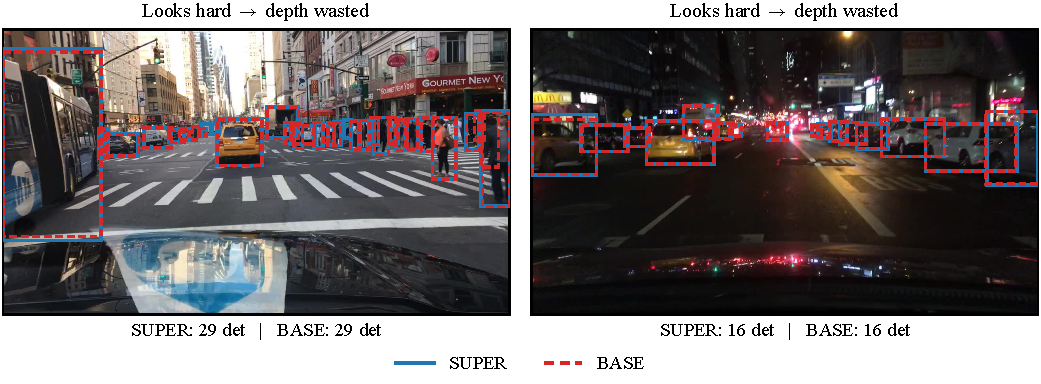
\includegraphics[width=0.96\textwidth]{fig_sample_routing.pdf}
\caption{
    The per-image benefit of the deep path is not predictable from how hard a
    scene looks to a human. \textbf{Left:} a cluttered daytime intersection;
    \textbf{Right:} a busy night scene---both look clearly difficult, yet the base path
    (dashed red) detects exactly as many objects as the super path (solid blue), with the
    boxes nearly coinciding ($29$ vs.\ $29$ and $16$ vs.\ $16$). In these visually hard
    scenes the extra depth is wasted---so semantic appearance (clutter, crowding,
    lighting) is a poor predictor of where the deep path actually pays off, motivating a
    learned per-image estimate of its benefit. Detections are from AnyDepth-YOLOv12s~\cite{kang2026anydepth} on BDD100K.
}
\label{fig:teaser}
\end{figure*}

\begin{table}[t]
\centering
\caption{Condition-stratified AP@[.50:.95] on the BDD100K validation set for the frozen AnyDepth-YOLOv12s. The benefit of deeper execution varies across inputs but is not well explained by broad semantic scene categories.}
\label{tab:condition_stratified}
\begin{tabular}{lrccc}
\toprule
Condition & $N$ & SUPER & BASE & Gap \\
\midrule
All & 10,000 & 33.23 & 32.05 & $+1.18$ \\
\midrule
\multicolumn{5}{l}{\emph{Time of day}} \\
\quad Daytime & 5,258 & 34.76 & 33.54 & $+1.22$ \\
\quad Night & 3,929 & 29.75 & 28.52 & $+1.23$ \\
\quad Dawn/Dusk & 778 & 33.28 & 32.22 & $+1.06$ \\
\midrule
\multicolumn{5}{l}{\emph{Weather}} \\
\quad Clear & 5,346 & 32.24 & 31.21 & $+1.03$ \\
\quad Overcast & 1,239 & 33.75 & 32.80 & $+0.96$ \\
\quad Rainy & 738 & 33.03 & 31.87 & $+1.16$ \\
\quad Snowy & 769 & 31.77 & 31.10 & $+0.66$ \\
\midrule
\multicolumn{5}{l}{\emph{Scene type}} \\
\quad Highway & 2,499 & 29.03 & 27.88 & $+1.15$ \\
\quad City street & 6,112 & 33.54 & 32.42 & $+1.13$ \\
\quad Residential & 1,253 & 38.00 & 36.66 & $+1.35$ \\
% \midrule
% \multicolumn{5}{l}{\emph{Crowd density}} \\
% \quad Low ($\le$ median) & 5,039 & 34.92 & 33.48 & $+1.44$ \\
% \quad High ($>$ median) & 4,961 & 32.46 & 31.43 & $+1.03$ \\
\bottomrule
\end{tabular}
\end{table}


Recent advances in dynamic detection have enabled a single model to operate under multiple computation regimes. 
In particular, AnyDepth-YOLO~\cite{kang2026anydepth} introduces a single detector that supports multiple executable paths with different computation depths, including a \emph{super} path (high accuracy, high computation) and a \emph{base} path (low computation with a modest accuracy drop).
This design enables input-dependent accuracy--efficiency trade-offs within a unified detector. 
While this provides the architectural and training foundations for dynamic execution, it does not address how to dynamically select the optimal execution depth for a given input, nor how to adjust these selections when the system's available compute or latency budget fluctuates.
A fundamental question therefore remains unresolved: \textit{how should one decide which execution depth to use for a given input under varying computation budgets?}


A natural intuition is that routing should follow semantic scene difficulty: visually complex scenes may require the super path, while simpler scenes are sufficient for the base path. 
However, Figure~\ref{fig:teaser} shows that this intuition does not reliably hold in practice. 
Even in visually challenging scenes, the performance gain from deeper execution can be negligible. 
Table~\ref{tab:condition_stratified} further demonstrates that the benefit of deeper execution remains consistent across broad semantic attributes such as time of day, weather, and scene type. 
For example, the SUPER--BASE performance gap is nearly identical between daytime and nighttime images ($+1.22$ vs.\ $+1.23$ AP), and remains similar across highway and city-street scenes ($+1.15$ vs.\ $+1.13$ AP). 
These observations suggest that semantic scene attributes are insufficient to characterize when deeper computation is beneficial, motivating a learned routing mechanism that estimates the expected benefit of additional depth on a per-image basis.


While the need for a learned per-image routing mechanism is clear, establishing an effective policy presents significant challenges. 
Conventional approaches to dynamic inference—primarily developed within the context of image classification—typically formulate routing as a discrete decision-making problem. 
These methods rely on efficiency-aware objectives that balance accuracy and computational cost, often implemented via Gumbel-Softmax relaxation~\cite{guo2019spottune, meng2020ar} or policy gradients~\cite{wu2018blockdrop}.
However, such approaches inherently embed a single accuracy–efficiency trade-off into the learned policy, effectively restricting it to a fixed operating regime determined by a trade-off coefficient, and making adaptation to different system budgets difficult without retraining. 
Moreover, the discrete optimization process is often unstable and prone to issues such as path collapse, requiring additional heuristics such as entropy regularization and carefully tuned balancing strategies. 
In contrast, routing path in object detection remains largely underexplored, and our goal is fundamentally different from these classification-oriented formulations. 
Rather than assigning each input to a single optimal execution path, we seek a routing mechanism that can adapt across varying latency and compute budgets, producing a spectrum of input-dependent routing behaviors rather than collapsing to a single solution.


To address this, we reformulate depth routing in object detection as an \emph{advantage regression} problem. With the detector weights frozen, the performance gain of executing the super path over the base path becomes a fixed, measurable quantity. 
This allows us to move beyond discrete policy learning; instead of treating routing as a stochastic decision-making process, we train a lightweight predictor to directly regress this per-image advantage from intermediate detector features. 
By transforming the problem into a standard supervised regression task, we eliminate the need for policy sampling, complex exploration strategies, and auxiliary collapse-prevention objectives.


At deployment, routing reduces to a simple threshold test on the predicted advantage. 
The threshold directly controls the accuracy--efficiency trade-off: lower values favor the \emph{super} path, whereas higher values route more inputs to the \emph{base} path. As a result, training becomes fully decoupled from deployment-time budget selection. A single trained router can realize a continuous spectrum of operating points through threshold sweeping alone, yielding an accuracy--efficiency trade-off curve without retraining or objective reweighting. Furthermore, because the operating point is governed by a single scalar threshold, the same router naturally supports online adaptation to time-varying latency budgets through lightweight feedback control.


Evaluations on KITTI, BDD100K, and Waymo Open tracking videos demonstrate that the proposed router achieves favorable accuracy--efficiency trade-offs with negligible overhead (under $0.003\%$ of the detector's computation).
The resulting router consistently outperforms heuristic baselines, delivering measurable reductions in latency and energy consumption while improving throughput.
At a sweet-spot operating point, it reduces per-frame computation, latency, and energy by roughly $12\%$ on KITTI and over $25\%$ on BDD100K with only a marginal 0.1 AP drop.
Moreover, the proposed formulation offers benefits beyond a single fixed operating point. 
By combining the router with a simple proportional--integral controller, the system can dynamically adapt the threshold on a frame-by-frame basis and track time-varying latency targets.
